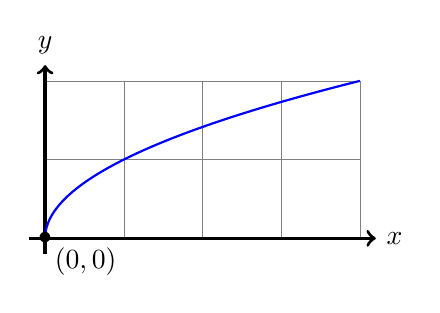
\begin{tikzpicture}
  \draw[very thin,color=gray] (0,0) grid (4,2);

  \draw[very thick,->] (-.2,0) -- (4.2,0) node[right] {$x$};
  \draw[very thick,->] (0,-0.2) -- (0,2.2) node[above] {$y$};
  
  \draw [color=blue,thick] plot[smooth,samples=500,domain=0:4] (\x,{sqrt(\x)});

  \node at (0,0) {$\bullet$};
  \node [below right] at (0,0) {$(0,0)$};
\end{tikzpicture}
